\clearpage
\subsection{Textual; Growing a Box}
\texHeader
\hypertarget{growBox tex}{}

\vspace*{0.5cm}

\begin{itemize}

\item[$\blacktriangleright$] In \texttt{grow}, create a simple control flow with one pattern. You'll want this pattern to match the invocation box with
\emph{any} two partitions, so create a bounded \texttt{this} box, and free \texttt{firstPartitionInBox} and \texttt{lastPartitionInBox} partitions.
You'll also need a creational variable to represent the new partition. The skeleton of your pattern should now resemble (Fig.~\ref{fig:growPattSkel}).

\vspace{0.5cm}

\begin{figure}[htbp]
\begin{center}
  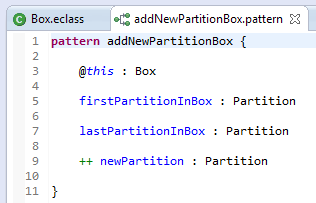
\includegraphics[width=0.5\textwidth]{eclipse_growPatternSkeleton}
  \caption{addPartitionsBox.pattern skeleton}
  \label{fig:growPattSkel}
\end{center}
\end{figure}

\item[$\blacktriangleright$] Next, we need to create an appropriate \emph{NAC} which will constrain the possible choices for \texttt{lastPartitionInBox}.
Create a \texttt{nextPartition} variable with an `!' operator preceding it immediately below \texttt{lastPartitionInBox}.

\vspace{0.5cm}

\item[$\blacktriangleright$] Now we need to establish the \texttt{next} links the pattern matcher will test. First, add \texttt{-> next : nextPartition}. This
command will attempt to establish a \texttt{next} reference from the current partition. Next, add \texttt{++ -> next: newPartition} (Fig.~\ref{fig:firstNAC}).
This line will only be reachable if the first (the NAC) fails! It establishes the newest element as the final partition.

\begin{figure}[htbp]
\begin{center}
  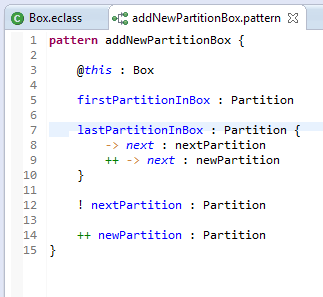
\includegraphics[width=0.5\textwidth]{eclipse_growLastNAC}
  \caption{Creating the first NAC}
  \label{fig:firstNAC}
\end{center}
\end{figure}

\vspace{0.5cm}

\item[$\blacktriangleright$] In a similar fashion create a second NAC for \texttt{firstPartitionInBox}. No new references have to be created here, so all you
need to establish is the check.

\begin{figure}[htp]
\begin{center}
  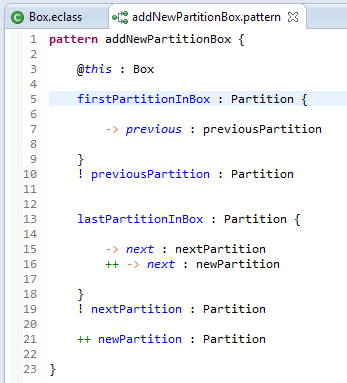
\includegraphics[width=0.55\textwidth]{eclipse_growFirstNAC}
  \caption{addPartitionsBox.pattern skeleton}
  \label{fig:growPattSkel}
\end{center}
\end{figure}

\clearpage

\item[$\blacktriangleright$] Fill in \texttt{@this} with appropriate references to the first and last partitions, then establish the \texttt{box} and
\texttt{previous} references in \texttt{newPartition} (Fig~\ref{fig:growAllLinks}).

\vspace{0.5cm}

\begin{figure}[htp]
\begin{center}
  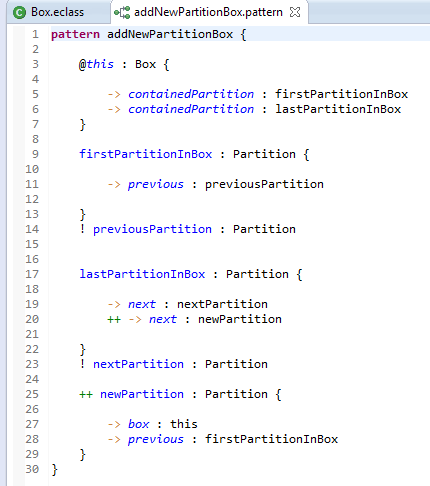
\includegraphics[width=0.65\textwidth]{eclipse_growLinks}
  \caption{A complete \emph{deterministic} pattern match}
  \label{fig:growAllLinks}
\end{center}
\end{figure}

\item[$\blacktriangleright$] We're not \emph{quite} done yet - our newest partition doesn't yet have a size. This means that not only do we need to make
another attribute contsraint, but \texttt{newPartition} needs to invoke a method in order to get the correct value. Call the method as you would in Java. 

\vspace{0.5cm}

\item[$\blacktriangleright$] Your workspace should now resemble Fig.~\ref{fig:patternComplete}

\begin{figure}[htp]
\begin{center}
  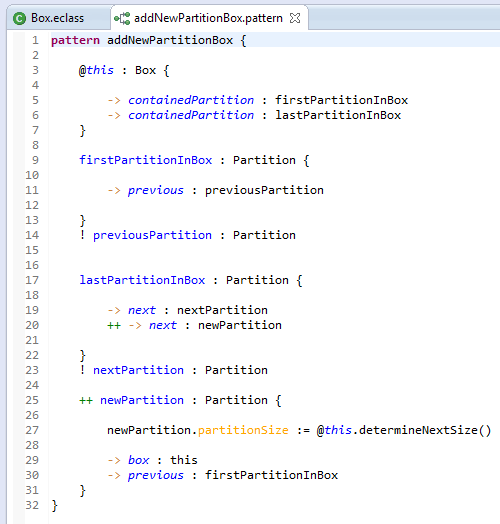
\includegraphics[width=0.9\textwidth]{eclipse_growFinished}
  \caption{Pattern complete!}
  \label{fig:patternComplete}
\end{center}
\end{figure}

\vspace{0.5cm}

\item[$\blacktriangleright$] That's everything! While NACs may have been difficult to understand at first, as you can see, they're not hard to implement, and
can be used in a wide variety of applications. To see how this method is implemented in the visual syntax, check out Fig~\ref{fig:sdm_grow_5} from the previous
section.

\end{itemize}